% Created 2020-06-19 sex 22:05
% Intended LaTeX compiler: pdflatex
\documentclass[11pt]{article}
\usepackage[utf8]{inputenc}
\usepackage[T1]{fontenc}
\usepackage{graphicx}
\usepackage{grffile}
\usepackage{longtable}
\usepackage{wrapfig}
\usepackage{rotating}
\usepackage[normalem]{ulem}
\usepackage{amsmath}
\usepackage{textcomp}
\usepackage{amssymb}
\usepackage{capt-of}
\usepackage{hyperref}
\usepackage{minted}
\usepackage[hyperref, x11names]{xcolor}
\hypersetup{colorlinks = true, urlcolor = SteelBlue4, linkcolor = black}
\usepackage[brazilian]{babel}
\author{Lourenço Henrique Moinheiro Martins Sborz Bogo - 11208005}
\date{\today}
\title{Exercícios 3 e 12 do capítulo 14}
\hypersetup{
 pdfauthor={Lourenço Henrique Moinheiro Martins Sborz Bogo - 11208005},
 pdftitle={Exercícios 3 e 12 do capítulo 14},
 pdfkeywords={},
 pdfsubject={},
 pdfcreator={Emacs 26.3 (Org mode 9.3.7)}, 
 pdflang={Brazilian}}
\begin{document}

\maketitle
\tableofcontents

\newpage
\section{Questão 3}
\label{sec:org7146402}
\paragraph{} Inicialmente foi necessário expandir, usando taylor até o termo a oitava, as seguintes expressões.
\begin{itemize}
\item \(f(x\pm h)\)
\item \(f(x\pm 2h)\)
\item \(f(x\pm 3h)\)
\end{itemize}
Somando as duas equações do primeiro item:
\begin{itemize}
\item \(f''(x) = \frac{f(x-h)-2f(x)+f(x+h)}{h^2} - \frac{h^2}{12}f^4(x) - \frac{h^4}{360}f^6(x) + O(h^6)\)
\end{itemize}
Somando as duas equações do segundo item:
\begin{itemize}
\item \(f''(x) = \frac{f(x-2h)-2f(x)+f(x+2h)}{4h^2} - \frac{h^2}{3}f^4(x) - \frac{2h^4}{45}f^6(x) + O(h^6)\)
\end{itemize}
Somando as duas equações do terceiro item:
\begin{itemize}
\item \(f''(x) = \frac{f(x-3h)-2f(x)+f(x+3h)}{9h^2} - \frac{3h^2}{4}f^4(x) - \frac{9h^4}{40}f^6(x) + O(h^6)\)
\end{itemize}

Agora temos 3 expressões para \(f''(x)\) cujo erro é O(h\textsuperscript{2}).

Usando a primeira e a segunda, obtemos:
\begin{itemize}
\item \(\frac{3f''(x)}{4} = \frac{f(x-h)-2f(x)+f(x+h)}{h^2} - \frac{f(x-2h)-2f(x)+f(x+2h)}{16h^2} + \frac{3h^4}{360}f^6(x) + O(h^6)\)
\end{itemize}
Usando a primeira e a terceira, obtemos:
\begin{itemize}
\item \(\frac{8f''(x)}{9} = \frac{f(x-h)-2f(x)+f(x+h)}{h^2} - \frac{f(x-3h)-2f(x)+f(x+3h)}{81h^2} + \frac{8h^4}{360}f^6(x) + O(h^6)\)
\end{itemize}

E juntando essas duas últimas expressões, conseguimos obter a expressão experada: 

\begin{itemize}
\item \(f''(x) = \frac{(2f(x-3h)-27f(x-2h)+270f(x-h)-490f(x)+270f(x+h)-27f(x+2h)+2f(x+3h))}{180h^2}\)
\end{itemize}

O algoritmo foi muito simples de implementar, apenas fiz uma função com essa expressão final e apliquei nela os valores pedidos.

\newpage
\section{Questão 12}
\label{sec:orgbf65cc2}

\paragraph{} Aqui, foi apenas uma questão de implementar a função que nos foi dada, calcular o erro nas condições pedidas e plotar num gráfico loglog.
\begin{figure}[htbp]
\centering
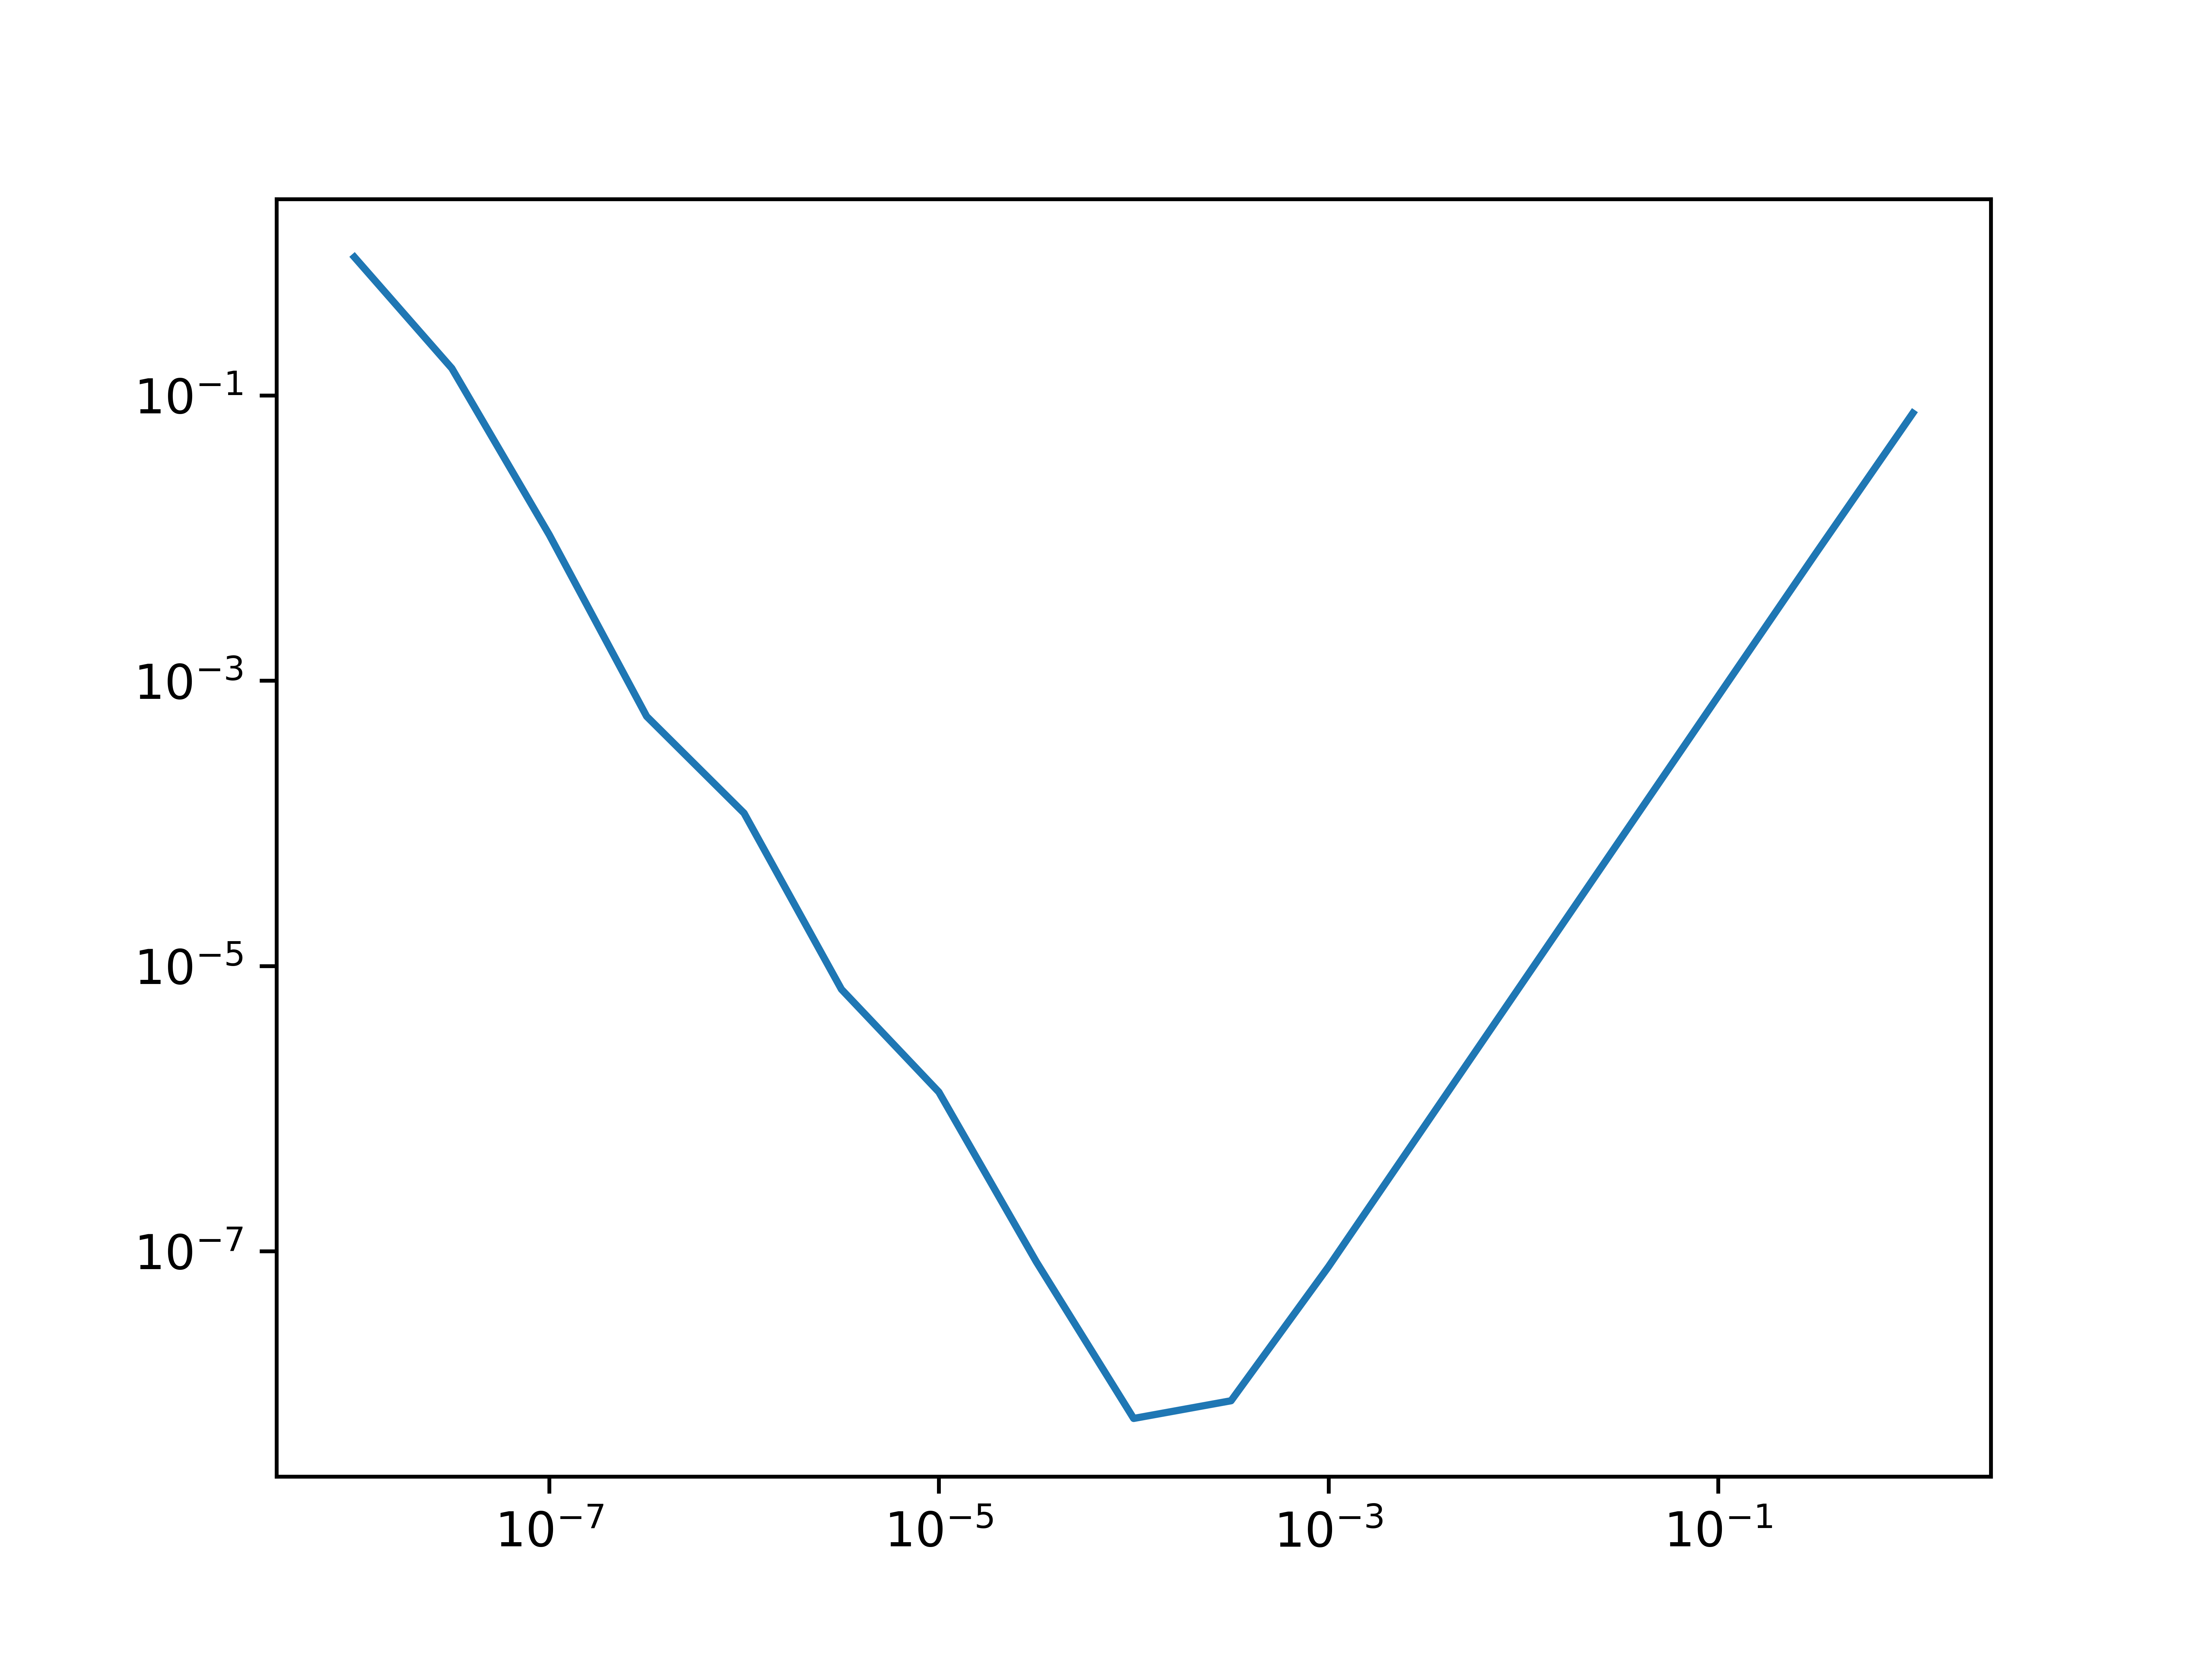
\includegraphics[width=.9\linewidth]{graph.png}
\caption{Gráfico loglog do erro}
\end{figure}

A explicação do gráfico é a seguinte: o erro tende a diminuir quanto mais diminuimos o h, o que pode ser evidenciado na metade direita do gráfico. O comportamento irregular que acontece no lado esquerdo se deve ao fato de que quando o h é muito pequeno, ocorre cancelamento catastrófico na conta, fazendo com que os erros de arredondamento dos pontos flutuantes fiquem maiores que o próprio erro do método de aproximação que estamos usando.
\end{document}